\section{History and Entanglement}
\label{sec:history-entanglement}

This section extends the verifiable state of \cref{sec:integrity-state} into a signed history of changes maintained by each \glslink{journal}{journal}. It also shows how independent organizations can link their histories so that each serves as evidence for the other, which \cref{sec:journal-web} later develops into access across the network.

\subsection{Connecting Independent Histories}

Organizations already exchange information through shared clouds, data lakes, APIs, replicated databases, signed documents, and ledgers. Each arrangement chooses a center of gravity, and each choice carries a corresponding limitation. A shared platform centralizes custody and policy, while replication multiplies copies of a single application state. Signed files travel independently but carry little context about succession, and webs of trust connect keys and attestations while leaving application data to other systems. Blockchain bridges transfer claims between consensus domains but inherit the complexity of both sides. However, many relationships do not cleanly fit any of these models. A manufacturer and buyer, laboratory and regulator, or publisher and archive each keep their own history, yet still need evidence that the other party's state existed before a later local event, even after the other party becomes unreachable. What is required, then, is a connection between histories that leaves each institution's governance intact. Secure timelines provide the starting point. A service repeatedly commits its state into a one-way succession, so later authenticators can establish the order of earlier states. Timeline \glslink{entanglement}{entanglement} carries signed authenticators across service boundaries and embeds them in other services' later authenticators~\cite{Maniatis2002timeline}. The embedding creates portable temporal mappings in which the past of one service becomes an input to the future of another. \glslink{synchronic-web}{Synchronic Web} \glslink{bridge}{bridges} apply that principle to histories whose states contain application \glslink{resource}{resources} and executable interpretation.

\subsection{Signed Local History}
\label{sec:signed-history}

Before journals can connect their histories, each must have a history to share. A journal builds it by turning local mutation into committed \glslink{step}{steps}. Applications accumulate a proposed state, inspect it, and then ask the journal to advance. The journal compares the proposal with the previous \glslink{head}{head} and stores transition metadata along with explicit inputs such as time and retained remote heads. It then binds its descriptor (the committed name, interface key, and endpoint through which others reach the journal) and key material into the new entry, constructs a canonical view of the chain with its signature fields blank, signs its \glslink{digest}{digest}, and advances the durable root. An authorized signing-key transition also requires a step, even when application state is unchanged, because the key that signs later heads is itself part of the committed history. Time, remote responses, randomness, and operator choices enter as explicit recorded values; anything the journal did not record cannot later be reproduced or verified. Applications that need exhaustive provenance, however, store event \glslink{object}{objects} or batch descriptions. \Cref{fig:step-anatomy} shows the logical result: application state, transition metadata, retained remote heads, time evidence, key-derivation and key-lineage material, and signatures share one integrity-protected tree built from the node structure of \cref{sec:minimal-structure}.\footnote{Reserved top-level names, marked with asterisks, separate application state (\texttt{*state*}) from journal-maintained structure.} \Cref{alg:commit-step} summarizes the commitment boundary: bind the \glslink{successor}{successor} state to its descriptors and any authorized key transition, sign the canonical view of the chain, and apply local retention policy without changing the logical history.

\begin{figure}[htbp]
  \centering
  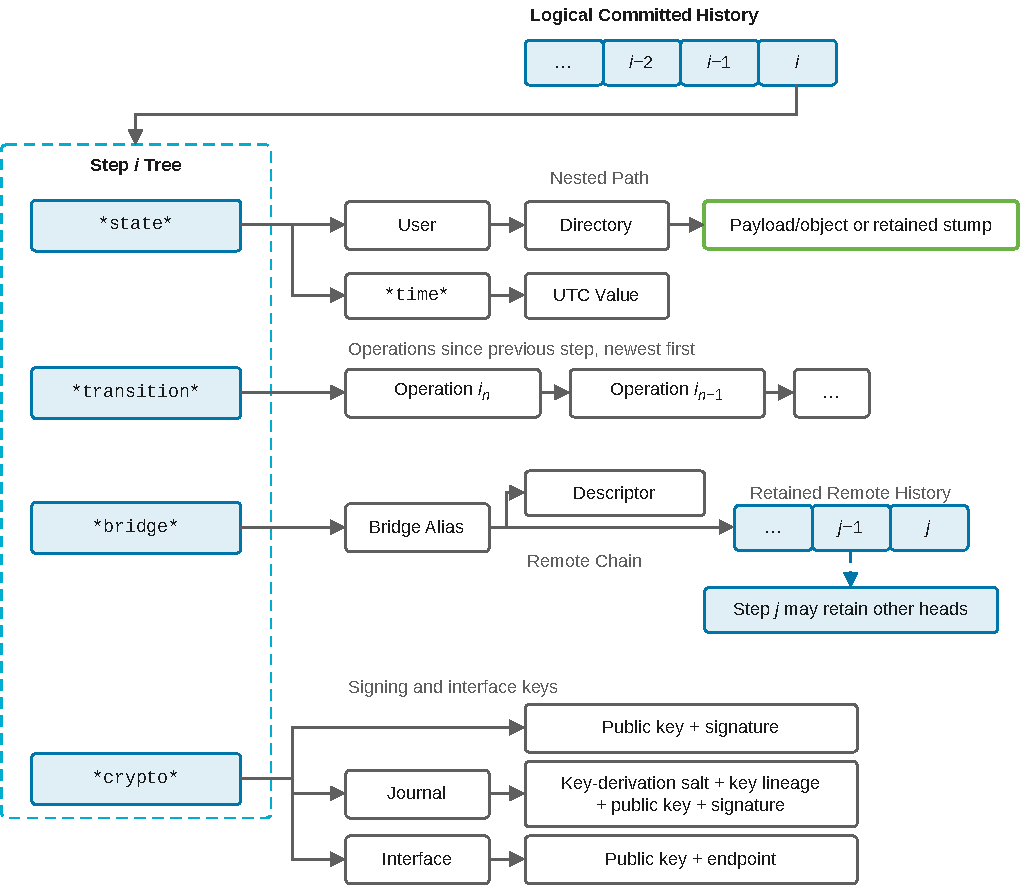
\includegraphics[scale=0.851]{figures/step-anatomy.pdf}
  \caption{Committed Step Anatomy}
  \label{fig:step-anatomy}
\end{figure}

\begin{algorithm}[htbp]
\caption{Commit Journal Step}
\label{alg:commit-step}
\begin{algorithmic}[1]
\Require Journal $J$, prepared time $t$, signing key pair $(p_k,s_k)$
\Ensure If state changed or a key transition is pending, a signed successor extends history and local retention is updated
\Function{CommitStep}{$J,t,p_k,s_k$}
  \State $(S,P,T) \gets \Call{JournalViews}{J}$ \Comment{Stage, permanent history, recent history.}
  \State $r \gets \Call{PendingKeyTransition}{J}$
  \State \Call{ValidateSigningContinuity}{$J,p_k,r$}
  \If{staged state is unchanged and no key transition is pending}
    \State \Return \Call{Size}{$P$}
  \EndIf
  \State $(S',H) \gets \Call{PrepareSuccessor}{S,t}$
  \State $C \gets \Call{Append}{P,H}$
  \State $C \gets \Call{BindDescriptorsAndKeyTransition}{C,J,r}$ \Comment{Written into the latest entry.}
  \State $C \gets \Call{BlankLatestSigningFields}{C}$
  \State $d \gets \Call{Digest}{\textproc{Node}(C)}$ \Comment{The enclosing chain is the signing object.}
  \State $\sigma \gets \Call{Sign}{s_k,d}$
  \State $P' \gets \Call{FillLatestSigningFields}{C,p_k,\sigma}$
  \State $(P',T') \gets \Call{ApplyRetentionPolicy}{J,P',T}$
  \Statex \Comment{Permanent: continuity, time, pins; recent: full state in window.}
  \State \Call{InstallSuccessor}{$J,S',P',T',r$}
  \State \Return \Call{Size}{$P'$}
\EndFunction
\end{algorithmic}
\end{algorithm}


Committed history grows without bound, so each journal must decide how much of it to keep. Historical identity and historical retention are separate choices, and keeping them separate is what makes long histories affordable. While a journal may retain recent heads in full, its permanent history keeps only chain continuity, signatures, selected proofs, and \glslink{pin}{pins}. \glslink{prune}{Pruning} replaces released material with \glslink{stump}{stumps}, using the partial-knowledge operations of \cref{sec:partial-knowledge-proof}. Pinning \glslink{merge}{merges} a chosen \glslink{slice}{slice} into the evidence held for a historical head, and unpinning releases that local obligation. A finite recent-history window therefore expresses a retention policy and makes no archival promise. Shrinking it immediately releases newly excluded unpinned material, while later widening changes future retention without reconstructing what was released. Each party preserves what serves its purpose and bears the cost of only that evidence. A buyer can pin an inspection report and its definitions, an archive can retain a complete site capture, and a witness can store signed heads and inclusion receipts. Related states share immutable structure, which reduces duplication, and replication and media renewal turn local retention into long-term availability.

\subsection{A Bridge Between Histories}
\label{sec:bridge-histories}

A bridge is a reciprocal signed-head-retention relationship. The journal that creates it becomes the sole ongoing synchronization initiator, and the acceptor returns its own signed head in the same exchange. Assigning that role to one side lets a private or intermittently reachable journal participate through outbound connections alone, while each journal keeps its commit cadence under local control. As shown in \cref{fig:bridge-reciprocal}, the initiator sends signed history and its descriptor under its current journal key. The acceptor verifies the sender's key lineage from its retained head, the committed endpoint, and that the new head extends the one already retained, before staging that head and returning corresponding evidence. The initiator performs the same checks locally, so neither side accepts evidence it has not verified itself. Each staged head enters the receiving journal's history at that journal's next local \texttt{step!}, and this inclusion orders the two histories. If B includes A's head $A_i$ in $B_j$, then $A_i$ precedes $B_j$, and $B_j$ with an inclusion proof serves as a portable receipt of that order. Because each journal commits on its own schedule, repeated exchange produces a weave of coarse ordering relations rather than a single global order, and each journal keeps its own sequence.

\begin{figure}[t]
  \centering
  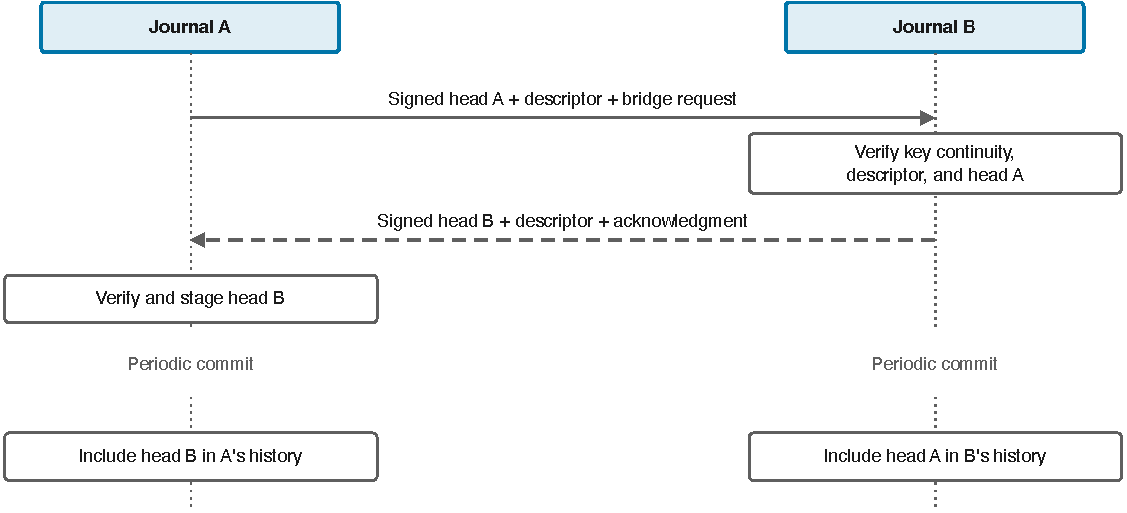
\includegraphics[scale=0.851]{figures/bridge-reciprocal-sequence.pdf}
  \caption{Bidirectional Head Exchange}
  \label{fig:bridge-reciprocal}
\end{figure}

Bridge operation also exposes practical controls. Synchronization cadence determines temporal resolution and network cost, and the bridge protocol determines the public material exchanged. Admission policy spans a range, from locked-down journals that accept incoming relationships only from preapproved signing keys, to open journals that may automatically accept any valid relationship.\footnote{Repeated synchronization safely confirms or advances acceptance, an already matching relationship can be re-checked read-only, and local stepping remains independent of remote traffic.}

\subsection{History at Network Scale}
\label{sec:network-history}

Sparse bridges turn entanglement into a network property. Because a remote head may itself contain other included heads, historical reachability composes recursively. From one selected journal, a verifier can follow retained heads across several relationships while preserving the path by which each piece of evidence became known. The result is a Web of historical viewpoints, each retaining its own timeline. This structure also governs how the network can grow. A ledger maintains one authoritative state for all participants, so every update that affects shared state must pass through a single consensus process and every full participant must process the updates of all others; the capacity of that consensus bounds the network~\cite{HarrisBraun2018holochain}. However, no single journal holds a globally authoritative state. Each is authoritative only for its own history and reaches agreement only with the journals it bridges, so its cost depends on its own activity and relationships rather than on the size of the network.

At this scale witnesses become central. A witness is any party, often another journal, that retains a journal's signed heads and compares them with the heads others received. Witnesses matter because nothing in the bridge protocol alone prevents a journal from signing distinct forks for journals that do not exchange evidence with each other. When witnesses compare heads or later histories include conflicting views, each journal retains the signed divergence as evidence. Transparency overlays and gossip develop this comparison as a general accountability technique~\cite{Chase2016transparency}. Each element plays a distinct role. Entangled journals contribute the retained remote heads, signatures establish authorship of each fork, and witness topology determines how quickly divergence becomes visible.

As these histories accumulate, object formats, \glslink{authorization}{authorization} rules, query languages, and application protocols will change on different schedules, and historical evidence remains most useful when the definitions needed to interpret it travel with the state itself. This change-management problem leads to the next layer, \glslink{self-encoding}{self-encoding} structure.
